\chapter{Herramientas matemáticas}

\section{Campos escalares y vectoriales }

Un \textbf{campo escalar} es una función que asigna a cada punto $(x,y)$ (o $(x,y,z)$) del espacio, un número real. Por ejemplo, en tres dimensiones $\phi = \phi(x,y,z)$. 

En Física, estas funciones son ocupadas, por ejemplo, para modelar la presión, $P(x,y,z)$, en cada punto de un fluido o la distribución de temperatura, $T(x,y,z)$, a través de un material. 

La gráfica de un campo escalar $\phi(x,y)$ puede ser representada en un gráfico tridimensional, de tal forma que a cada punto del plano $xy$ se le asigna un valor en el eje $z$. Matemáticamente, son todas las ternas $(x,y,z)$ con $z = \phi(x,y)$. 

\begin{ejemplo}
    Consideremos la función paraboloide hiperbólico
    $$z = \phi(x,y) = x^2+y^2,$$

    cuyas gráficas en 3-D y curvas de nivel, esto es, curvas
    $$\phi(x,y) = k,$$

    para una cierta constante $k \in \mathbb{R}$, se 
    detallan en la figura \ref{fig:CampoEscalar}.

    \begin{figure}[H]
        \centering
        \subfigure[]{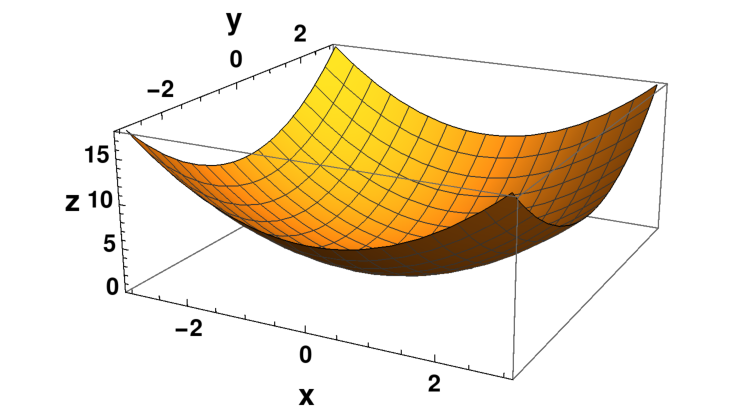
\includegraphics[width=0.46\textwidth]{Figuras/CampoEscalar.pdf}} \hspace{1cm}
        \subfigure[]{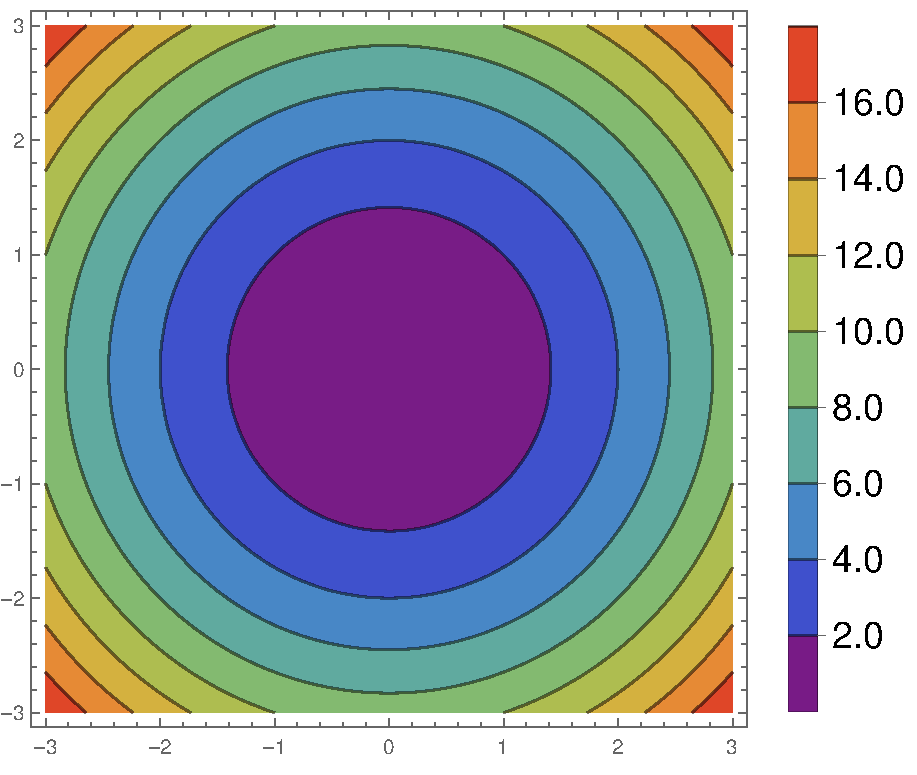
\includegraphics[width=0.35\textwidth]{Figuras/CurvasNivel.pdf}} 
        \caption{En (a), la gráfica del paraboloide $z = x^2+y^2$; y en (b), la gráfica de las curvas de nivel del paraboloide.}
        \label{fig:CampoEscalar}
    \end{figure}
\end{ejemplo}

Por otro lado, para campos escalares $\phi(x,y,z)$, no es posible tener una representación gráfica debido a que la gráfica de la función vive en un espacio de  cuatro dimensiones, pues, bajo la misma lógica del campo $\phi(x,y)$, un punto de la gráfica sería la $4$-tupla $(x,y,z,w) \in \mathbb{R}^4$, con $w = \phi(x,y,z)$. 

 
Un \textbf{campo vectorial} en el espacio de dos (o tres) dimensiones, es una función $\vec{V}$ que asigna a cada punto $(x,y)$ (o $(x,y,z)$) del espacio, un vector en dos (o tres) dimensiones dado por $\vec{V}(x,y)$ (o $\vec{V}(x,y,z)$).

Usando la base canónica de $\mathbb{R}^2$ y $\mathbb{R}^3$: $\{\hat{x},\hat{y}\}$ y $\{\hat{x},\hat{y}, \hat{z}\}$,  respectivamente. La notación para el campo vectorial $\vec{V}$ está dada por:
\begin{align*}
    \vec{V} (x,y) &= V_x(x,y) \hat{x} + V_y(x,y) \hat{y}, \\
    \vec{V}(x,y,z) &= V_x(x,y,z) \hat{x} + V_y(x,y,z) \hat{y} + V_z(x,y,z) \hat{z},   
\end{align*}

donde $V_x, V_y$ y $V_z$ son campos escalares.

Es habitual graficar las campos vectoriales dibujando en cada punto $(x,y)$ (o $(x,y,z)$) del espacio el vector $\Vec{V}(x,y)$ (o $\Vec{V}(x,y,z)$).

\begin{ejemplo}
\ 

    \begin{itemize}
        \item $\vec{V}(x,y) = -y \hat{x} + x \hat{y}$.

        \begin{figure}[H]
            \centering
            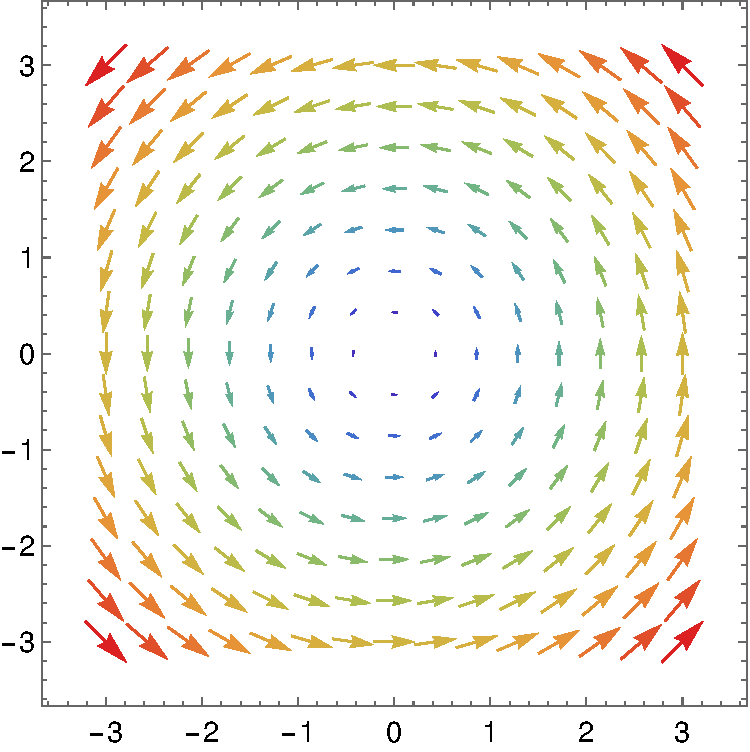
\includegraphics[scale = 0.45]{Figuras/CampoVectorial1.pdf}
            \caption{Gráfica del campo $\vec{V}(x,y) = -y \hat{x} + x \hat{y}$.}
            \label{fig:Campo_Vectorial1}
        \end{figure}

        \item Campo en tres dimensiones con simetría radial: $\vec{V}(x,y,z) = x \hat{x} + y \hat{y} + z \hat{z}$.

        \begin{figure}[H]
            \centering
            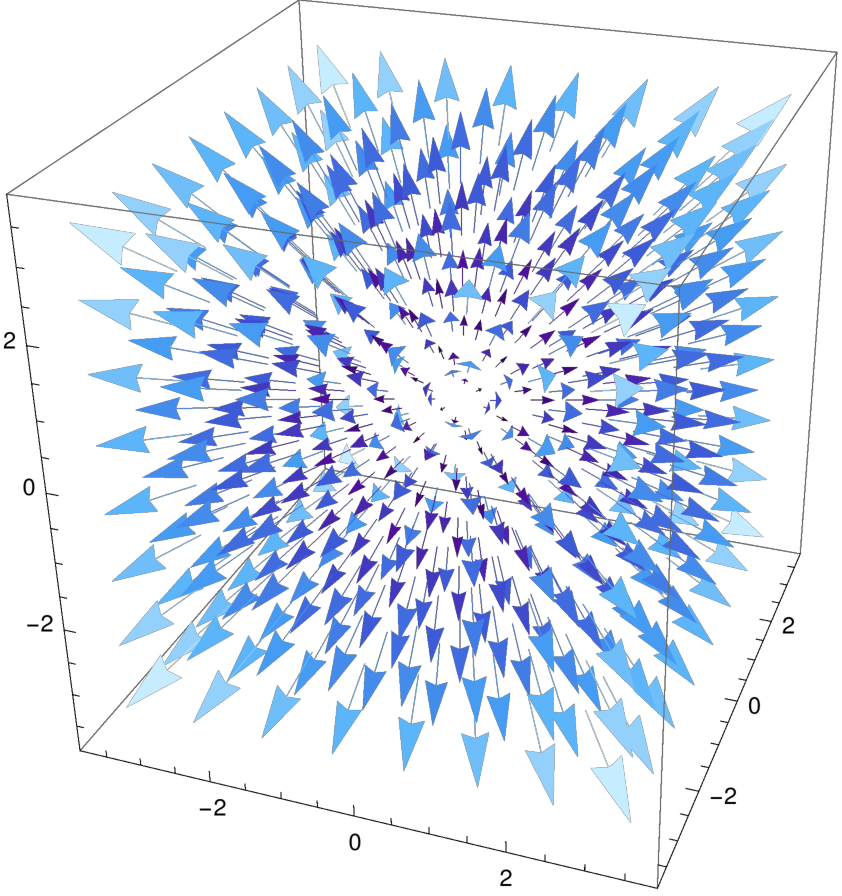
\includegraphics[scale = 0.44]{Figuras/CampoVectorial2.pdf}
            \caption{Gráfica del campo  $\vec{V}(x,y,z) = x \hat{x} + y \hat{y} + z \hat{z}$.}
            \label{fig:Campo_Vectorial2}
        \end{figure}
    \end{itemize}
\end{ejemplo}

\section{Operadores vectoriales} \label{Operadores}

Sea la función de una variable real: $f(x)$. De los primeros cursos de Cálculo sabemos que si $f$ es derivable, la derivada $df/dx$ nos indica cómo cambia $f(x)$ con respecto $x$, geométricamente, corresponde a la pendiente de la gráfica $y = f(x)$. 

Si consideramos cantidades infinitesimales,
$$df = \left(\frac{df}{dx} \right) dx.$$

En palabras: Si incrementamos $x$ por una cantidad infinitesimal $dx$, entonces $f$ cambia por una cantidad $df$; la derivada es el factor de proporcionalidad.

\subsection*{Gradiente de un campo escalar}

Si consideramos ahora una función de tres variables: $f(x,y,z)$. Nos gustaría generalizar la noción de “derivada” de la función, que no depende de una sino de tres variables.

Una derivada debería decirnos cuán rápido una función cambia, para el caso de tres variables la situación es más complicada porque ya no tenemos solo una dirección en un eje para evaluar el cambio, sino varias direcciones (representadas como vectores en $\mathbb{R}^3$). 

Definimos, artesanalmente, la derivada parcial de $f(x,y,z)$ con respecto al eje $x_i$,
$$\frac{\partial f}{\partial x_i}, \quad \text{con} ~ x_i = x,y,z,$$

como la “variación” de $f$ con respecto a la dirección dada por el eje $x_i$, manteniendo el resto de las variables constantes. Por ejemplo, 
$$\frac{\partial}{\partial y}[2xy] = 2x,$$

donde hemos derivado suponiendo que $x$ es una constante.

Para saber cuánto varía $f$ cuando nos trasladamos un diferencial de posición $d\Vec{x} = dx \, \hat{x} + dy \,\hat{y} + dz \,\hat{z}$, el Cálculo en varias variables nos entrega el siguiente teorema:
$$df = \left(\frac{\partial f}{\partial x}\right) dx + \left(\frac{\partial f}{\partial y}\right) dy +\left(\frac{\partial f}{\partial z}\right) dz.$$

Note que sólo nos bastó definir tres derivadas parciales para cuantificar el cambio infinitesimal de $f$, lo cual se justifica debido a que el espacio tridimensional $\mathbb{R}^3$ sólo tiene tres direcciones linealmente independientes.

Notemos que 
\begin{align*}
    df &= \left( \frac{\partial f}{\partial x} \hat{x} +  \frac{\partial f}{\partial y} \hat{y} +  \frac{\partial f}{\partial z} \hat{z}\right)  \cdot (dx \, \hat{x} + dy \, \hat{y} + dz \, \hat{z})\\
    &= (\Vec{\nabla} f) \cdot (d\Vec{x}),
\end{align*}

donde 
\begin{shaded}
$$\vec{\nabla}f(x,y,z) := \frac{\partial f}{\partial x} \hat{x} + \frac{\partial f}{\partial y} \hat{y} +  \frac{\partial f}{\partial z} \hat{z}$$
\end{shaded}

es el \textbf{gradiente de $f$} (en coordenadas cartesianas).

\textbf{Nota:} Lo expuesto es cierto si $f(x,y,z)$ es un campo escalar diferenciable. \footnote{$f(x,y,z)$ se dice diferenciable si es posible aproximar la gráfica de la función en cada punto por un plano tangente a la gráfica. Además,  garantiza la existencia de las derivadas parciales.}

Si omitimos la función $f$, podemos definir el \textbf{operador nabla}:
\begin{shaded}
$$\vec{\nabla} :=  \hat{x} \frac{\partial}{\partial x} +  \hat{y} \frac{\partial}{\partial y} +   \hat{z} \frac{\partial}{\partial z}.$$
\end{shaded}

El vector gradiente tiene dos \underline{interpretaciones geométricas} importantes:

\begin{enumerate}
\item En tres dimensiones, $\vec{\nabla}f(x,y,z)$ es un vector normal al plano tangente a la superficie $f ( x, y, z ) = C$ en cada punto. Para el caso de dos dimensiones, $\vec{\nabla}f(x,y)$ es un vector normal a la recta tangente a la curva $f(x,y) = C$.

\begin{figure}[H]
    \centering
    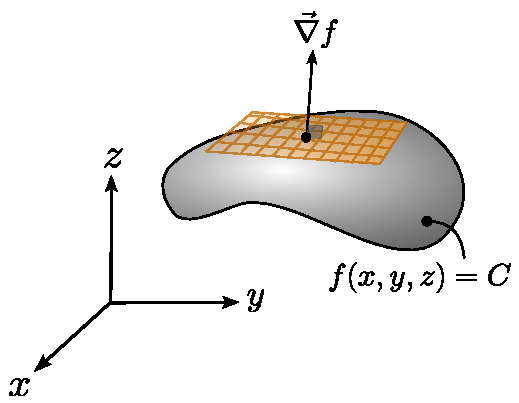
\includegraphics[scale = 0.8]{Figuras/Gradiente1.pdf}
    \caption{El gradiente como vector normal a la superficie $f(x,y,z) = C$.}
    \label{fig:Gradiente1}
\end{figure}

\item En dos dimensiones, $\vec{\nabla}f(x_0,y_0)$  indica la dirección del máximo incremento de $f(x,y)$ en el punto $(x_0,y_0)$. Para el caso de tres dimensiones, $\vec{\nabla}f(x_0,y_0,z_0)$  indica la dirección del máximo incremento de $f(x,y,z)$ en el punto $(x_0,y_0,z_0)$. 

\begin{figure}[H]
    \centering
    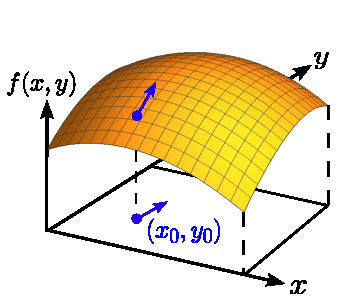
\includegraphics[scale = 0.89]{Figuras/Gradiente2.pdf}
    \caption{El gradiente como dirección de máximo incremento de $f(x,y)$ en $(x_0,y_0)$.}
    \label{fig:Gradiente2}
\end{figure}

\end{enumerate}

\begin{ejemplo}
    Determine el vector normal a la esfera $x^2+y^2+z^2 = 3$ en el punto $(1,1,1)$.

    \textbf{Solución:} Sea $f(x,y,z) = x^2+y^2+z^2$, 
    \begin{align*}
        \frac{\partial f}{\partial x} &= \frac{\partial}{\partial x}[x^2] + \cancelto{0}{\frac{\partial}{\partial x}[y^2]} + \cancelto{0}{\frac{\partial}{\partial x}[z^2]} = 2x,   \\
        \frac{\partial f}{\partial y} &=\cancelto{0}{\frac{\partial}{\partial y}[x^2]} + \frac{\partial}{\partial y}[y^2] + \cancelto{0}{\frac{\partial}{\partial y}[z^2]} = 2y, \\
        \frac{\partial f}{\partial z} &=\cancelto{0}{\frac{\partial}{\partial z}[x^2]} + \cancelto{0}{\frac{\partial}{\partial z}[y^2]} + \frac{\partial}{\partial z}[z^2]  = 2z.
    \end{align*}

    Luego, el gradiente de $f$ es
    $$\Vec{\nabla} f(x,y,z) = 2x \hat{x} + 2y \hat{y} + 2z \hat{z}.$$

    Por lo tanto, el vector normal a la esfera en $(1,1,1)$ es $\Vec{\nabla} f(1,1,1) = 2 \hat{x} + 2 \hat{y} + 2 \hat{z}.$
\end{ejemplo}

\subsection*{Divergencia de un campo vectorial}

Para un campo vectorial
$$\vec{V} (x,y,z) = V_x(x,y,z) \hat{x} + V_y(x,y,z) \hat{y} + V_z(x,y,z) \hat{z} ,$$

la \textbf{divergencia} está definida por
\begin{shaded}
    $$\mbox{div} ~\vec{V} \equiv \vec{\nabla} \cdot \vec{V} := \frac{\partial V_x}{\partial x} + \frac{\partial V_y}{\partial y} + \frac{\partial V_z}{\partial z}.$$
\end{shaded}

\textbf{Nota:} Cualquier campo vectorial para el cual $\vec{\nabla} \cdot \vec{V} = 0$ se dice que es \textit{solenoidal}.

Diremos que la divergencia puede ser considerada como una medida cuantitativa de cuanto un campo vectorial “diverge” o “converge” en un punto dado. 

\begin{figure}[H]
    \centering
    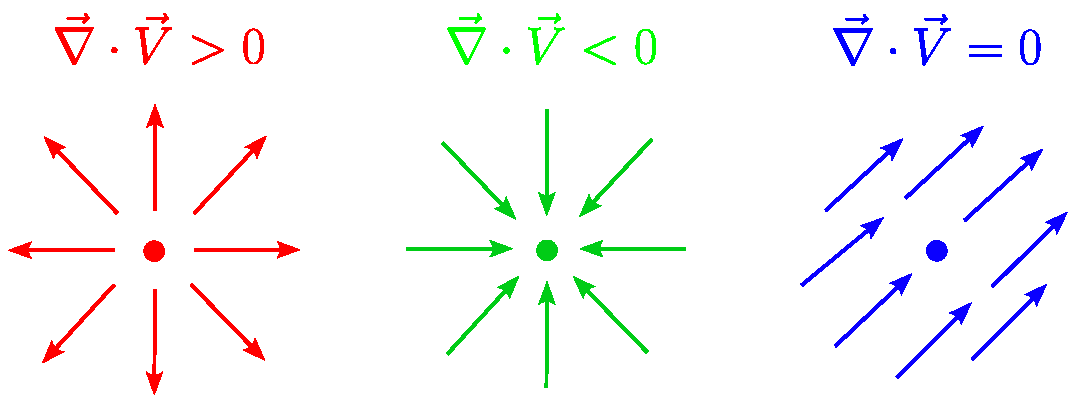
\includegraphics[scale = 0.55]{Figuras/Divergencia.pdf}
    \caption{Interpretación física de la divergencia.}
    \label{fig:sign_divergence}
\end{figure}

Analicemos los tres posibles casos:

\begin{enumerate}
\item Si $\vec{\nabla} \cdot \vec{V} >0$ en algún punto, estamos en presencia de una \textit{fuente} o \textit{manantial} desde donde el campo vectorial radia hacia el exterior. 

\item Si $\vec{\nabla} \cdot \vec{V} < 0$ estamos en presencia de un \textit{sumidero} pues el campo “converge” hacia dicho  punto.

\item  Si $\vec{\nabla} \cdot \vec{V} =0$ el campo no converge ni diverge (no hay fuentes ni sumideros); no pueden tener extremos localizados, las líneas solo pueden ser cerradas, o ir del infinito o al infinito, o dar vueltas sobre sí mismas, sin llegar a cerrarse.
\end{enumerate}

\begin{ejemplo}
    En mecánica de fluidos, la distribución de las velocidades del fluido es descrita por un campo vectorial $v(x, y, z, t)$. Esto representa la velocidad del fluido en el punto $(x, y, z)$ en el instante $t$. En nuestro caso omitiremos la dependencia temporal. Suponga que el campo de velocidades de un fluido es
    $$\Vec{v}(x,y) = (x^2-y^2) \hat{x} + 2xy \hat{j}$$

    \begin{figure}[H]
    \centering
    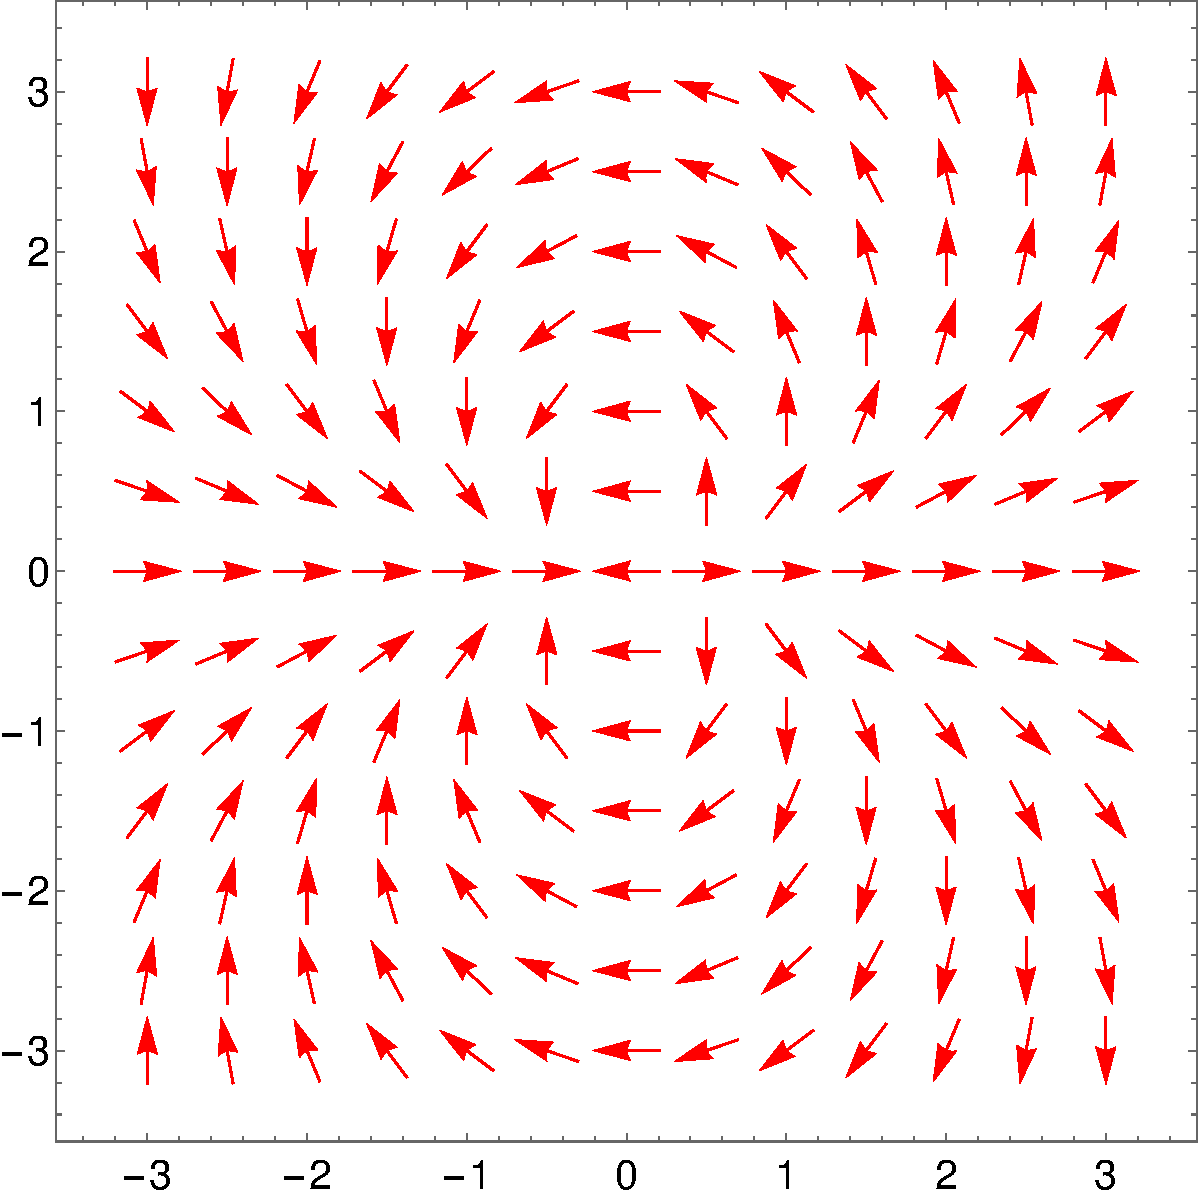
\includegraphics[scale = 0.3]{Figuras/Ej-Divergencia}
    \caption{Gráfica del campo de velocidades $\Vec{v}(x,y) = (x^2-y^2) \hat{x} + 2xy \hat{j}$ normalizado.}
    \label{fig:Ej_Divergencia}
    \end{figure}

    Calcule la divergencia y determine si en el punto $(1,2)$ es más una fuente o sumidero.

    \textbf{Solución:} La divergencia está dada por
    $$\vec{\nabla} \cdot \Vec{v} = \frac{\partial}{\partial x}[x^2-y^2] + \frac{\partial}{\partial y}[2xy] = 2x+2x = 4x. $$

    En el punto $(1,2)$, $\vec{\nabla} \cdot \Vec{v}(1,2) = 4 > 0$. Por lo tanto, en este punto se tiene más una fuente que un sumidero. Físicamente, la densidad del fluido decrece en ese punto.
\end{ejemplo}
  

\subsection*{Rotacional de un campo vectorial}

Sea el campo vectorial
$$\vec{V} (x,y,z) = V_x(x,y,z) \hat{x} + V_y(x,y,z) \hat{y} + V_z(x,y,z) \hat{z}.$$

El \textbf{rotor} (o \textbf{rotacional}) de $\vec{V}$ está definido por 
\begin{shaded}
 $$\mbox{rot} ~ \vec{V} := \left( \frac{\partial V_z}{\partial y} - \frac{\partial V_y}{\partial z} \right) \hat{x} + \left( \frac{\partial V_x}{\partial z} - \frac{\partial V_z}{\partial x} \right) \hat{y} + \left( \frac{\partial V_y}{\partial x} - \frac{\partial V_x}{\partial y} \right) \hat{z}.$$   
\end{shaded}

Otra forma de expresar el rotacional de un campo vectorial es
\begin{shaded}
$$\mbox{rot} ~ \vec{V} \equiv \vec{\nabla} \times \vec{V} = \left| \begin{array}{ccc}
\hat{x} & \hat{y} & \hat{z}  \\
\frac{\partial}{\partial x} & \frac{\partial}{\partial y} & \frac{\partial}{\partial z}  \\
V_x & V_y & V_z
\end{array} \right|.$$  
\end{shaded}

El rotor asociado a un campo vectorial $\vec{V}$ es otro campo vectorial, y por tanto el rotor calculado en un punto es un vector. El \textit{rotor} es un operador vectorial $(\vec{\nabla} \times)$ que muestra la tendencia de un campo vectorial a inducir una rotación alrededor de un punto.

Si el rotor de un campo vectorial es cero en un punto significa que el campo vectorial no tiene rotaciones en ese punto (\textit{campo irrotacional}). En cambio si el rotor es distinto de cero significa que el campo tiene circulación o remolinos. En la siguiente figura se ilustra los dos casos para un campo vectorial $\Vec{V}$.

\begin{figure}[H]
    \centering
    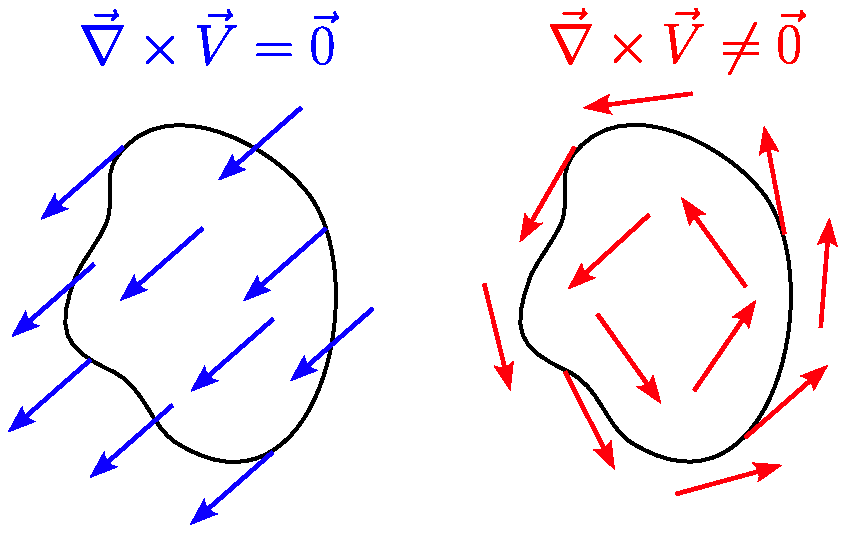
\includegraphics[scale = 0.52]{Figuras/Rotor.pdf}
    \caption{Interpretación física del rotacional.}
    \label{fig:rotor}
\end{figure}

\begin{ejemplo}
    Consideremos el campo vectorial
    $$\Vec{F}(x,y,z) = y \hat{x} - x\hat{y}.$$
    
    El rotor está dado por
    
    $$\vec{\nabla} \times \vec{F} = \left| \begin{array}{ccc}
    \hat{x} & \hat{y} & \hat{z}  \\
    \frac{\partial}{\partial x} & \frac{\partial}{\partial y} & \frac{\partial}{\partial z}  \\
    y & -x & 0
    \end{array} \right| = 0 \hat{x} + 0 \hat{y} + \left( \frac{\partial}{\partial x}[-x] - \frac{\partial}{\partial y} [y]\right) \hat{z} = -2 \hat{z}.$$ 

    \begin{figure}[H]
        \centering
        \subfigure[]{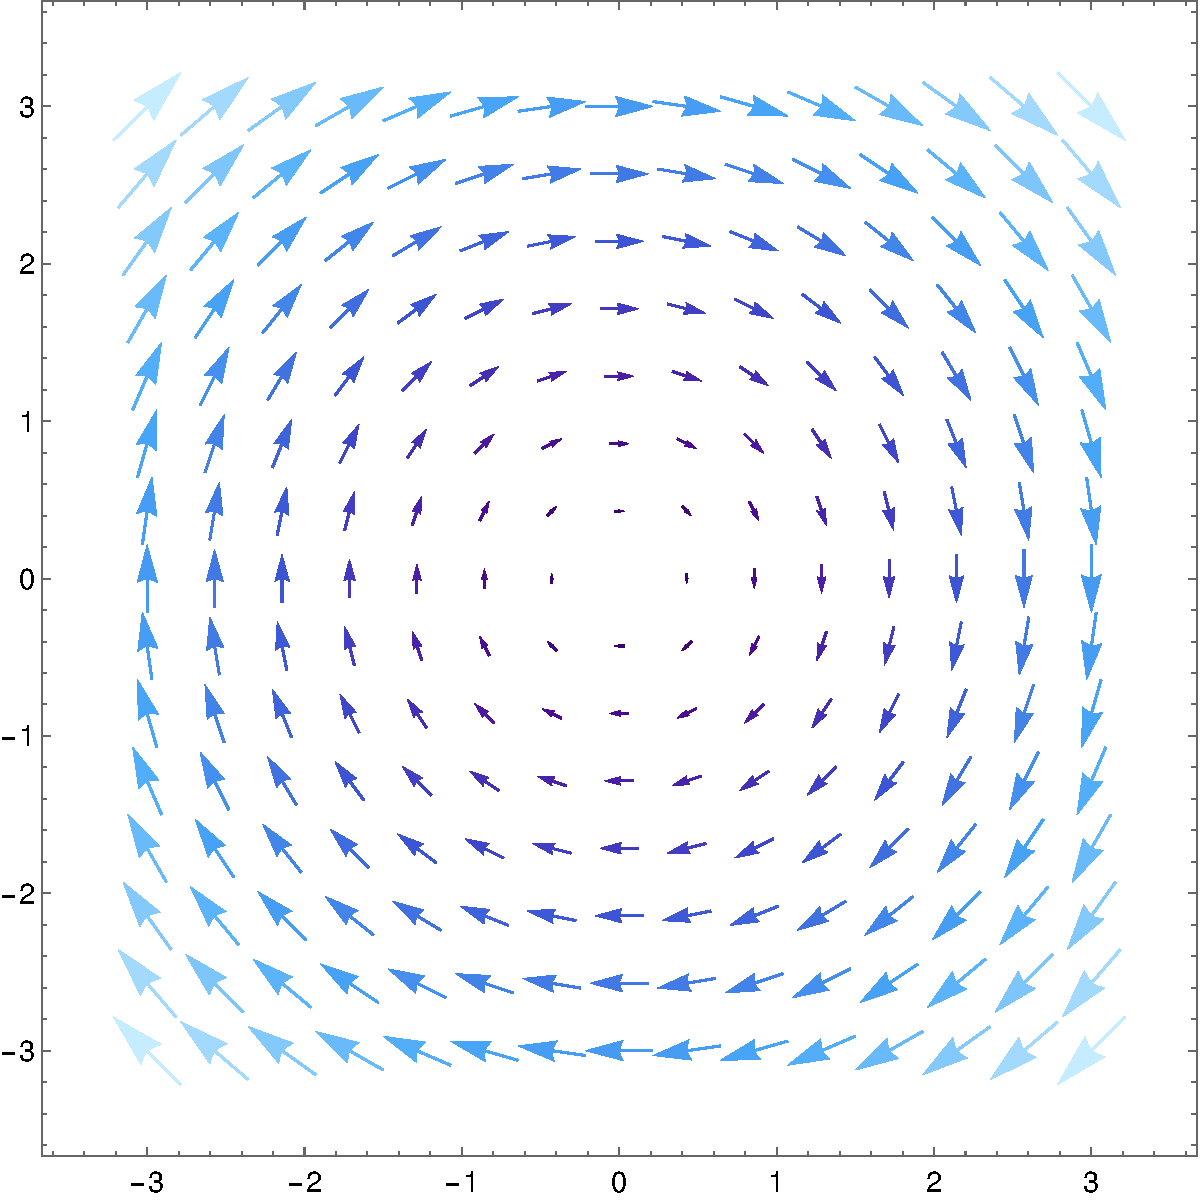
\includegraphics[width=0.36\textwidth]{Figuras/Ej-Rotor-1.pdf}} \hspace{1cm}
        \subfigure[]{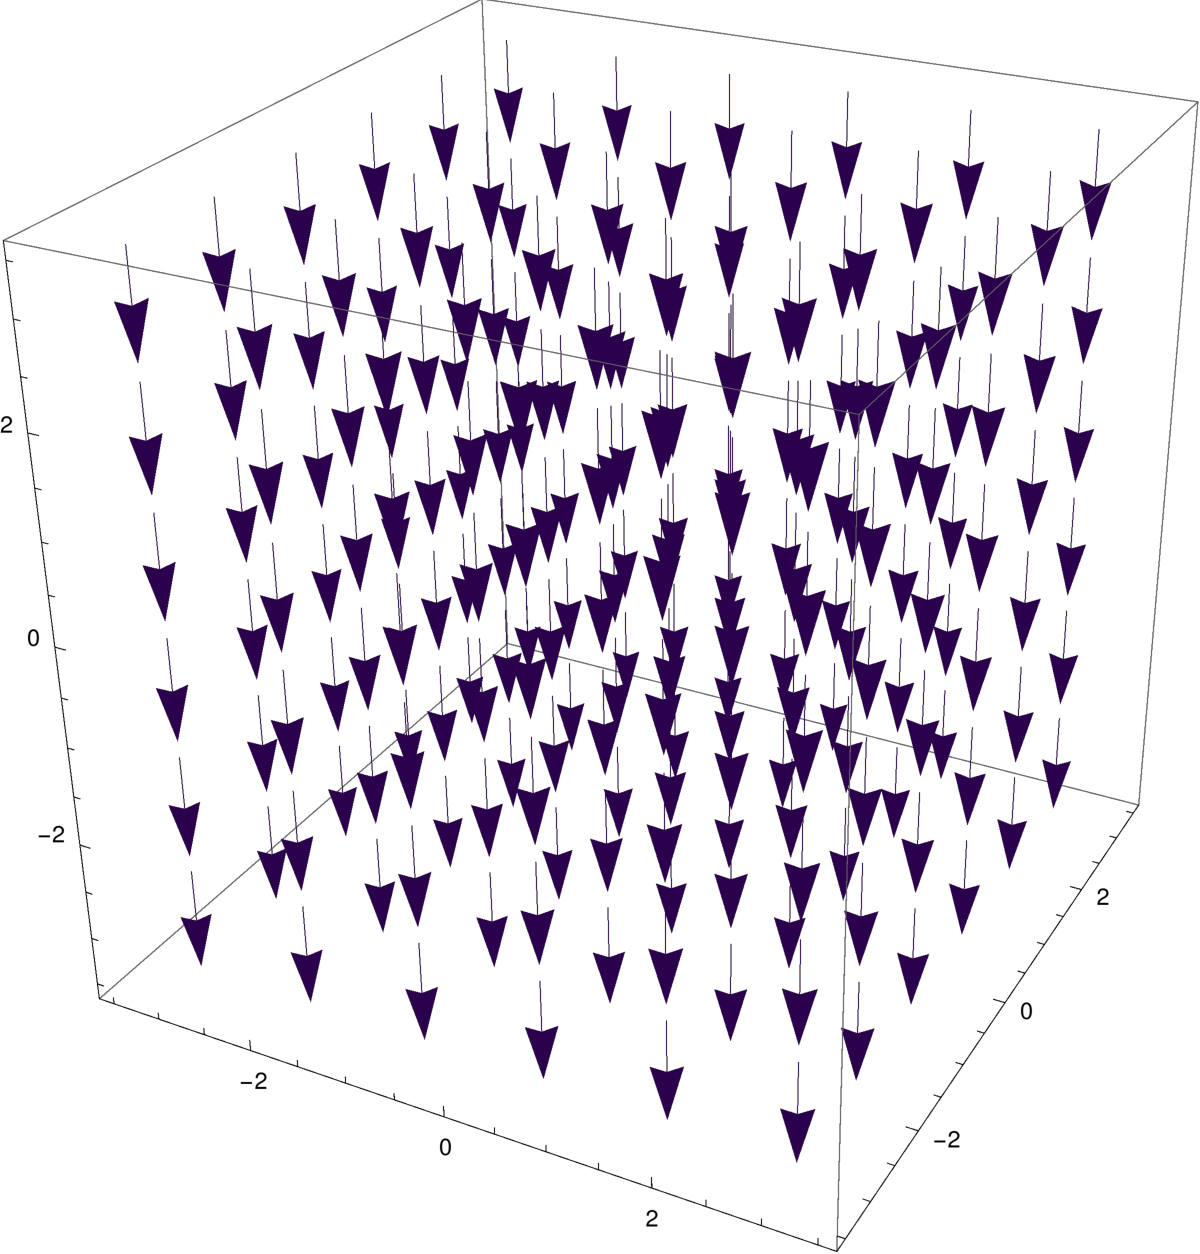
\includegraphics[width=0.36\textwidth]{Figuras/Ej-Rotor-2.pdf}} 
        \caption{Gráfica del campo vectorial $\Vec{F}(x,y,z) = y \hat{x} - x\hat{y}$ (a) y su rotacional (b).}
        \label{fig:Ej_Rotor}
    \end{figure}
    
    El campo vectorial resultante describe que la circulación en todos los puntos será en torno de la dirección del eje $z$ negativo. Además, al ser un campo vectorial uniforme, el objeto descrito antes tendrá la misma intensidad del rotacional independiente de donde se sitúe.
\end{ejemplo}

\subsection*{Laplaciano}

En muchas aplicaciones Físicas aparecen ciertas combinaciones del gradiente, la divergencia y el rotacional. Una de ellas es la divergencia de un gradiente.

Sea $f(x,y,z)$ un campo escalar diferenciable:
\begin{align*}
    \vec{\nabla} \cdot \vec{\nabla} f &=  \left( \hat{x} \frac{\partial}{\partial x}  + \hat{y} \frac{\partial}{\partial y}   + \hat{z}\frac{\partial}{\partial z}  \right) \cdot \left( \frac{\partial f}{\partial x} \hat{x} + \frac{\partial f}{\partial y} \hat{y} + \frac{\partial f}{\partial z} \hat{z} \right) \\
&= \frac{\partial^2 f }{\partial x^2} + \frac{\partial^2 f}{\partial y^2} + \frac{\partial^2 f}{\partial z} .  
\end{align*}

De aquí definimos el \textbf{Laplaciano} de $f$ como
\begin{shaded}
    $$\nabla^2 f := \frac{\partial^2 f }{\partial x^2} + \frac{\partial^2 f}{\partial y^2} + \frac{\partial^2 f}{\partial z^2}.$$
\end{shaded}

\subsection*{Propiedades de los operadores vectoriales}

\begin{teorema} \label{Prop-Op-Vect}
Sean $\Vec{A}$ y $\Vec{B}$ dos campos vectoriales diferenciables y, $\phi$ y $\psi$ dos campos escalares diferenciables de $(x,y,z)$. Entonces,
\begin{enumerate}
    \item $\Vec{\nabla}(\phi + \psi) = \Vec{\nabla} \phi + \Vec{\nabla} \psi$.

    \item $\Vec{\nabla} \cdot (\vec{A} + \Vec{B}) = \Vec{\nabla} \cdot \Vec{A} + \Vec{\nabla} \cdot \Vec{B}$.

    \item $\Vec{\nabla} \times (\vec{A} + \Vec{B} ) = \Vec{\nabla} \times \Vec{A} + \Vec{\nabla} \times \Vec{B}$.

    \item $\Vec{\nabla} \cdot (\phi \Vec{A}) = (\Vec{\nabla} \phi) \cdot \Vec{A} + \phi (\Vec{\nabla} \cdot \Vec{A})$.

    \item $\Vec{\nabla} \times (\phi \Vec{A}) = (\Vec{\nabla} \phi) \times \Vec{A} + \phi(\Vec{\nabla} \times \Vec{A})$.

    \item $\Vec{\nabla} \cdot (\Vec{A} \times \Vec{B}) = \Vec{B} \cdot (\Vec{\nabla} \times \Vec{A}) - \Vec{A} \cdot (\Vec{\nabla} \times \Vec{B})$.

    \item $\Vec{\nabla} \times (\Vec{A} \times \Vec{B}) = (\Vec{B} \cdot \Vec{\nabla}) \Vec{A} - (\Vec{A} \cdot  \Vec{\nabla}) \Vec{B} + \Vec{A}( \Vec{\nabla} \cdot \Vec{B}) - \Vec{B}( \Vec{\nabla} \cdot \Vec{A})$.

    \item $ \Vec{\nabla}(\Vec{A} \cdot \Vec{B}) = (\Vec{B}  \cdot \Vec{\nabla}) \Vec{A} + (\Vec{A} \cdot  \Vec{\nabla}) \Vec{B} + \Vec{A} \times ( \Vec{\nabla} \times \Vec{B}) + \Vec{B} \times ( \Vec{\nabla} \times \Vec{A})$.

    \item Si $\phi$ es de clase $C^2$, $\vec{\nabla} \times  \Vec{\nabla} \phi = \Vec{0}$.

    \item Si $\Vec{A}$ es de clase $C^2$, $\vec{\nabla} \cdot  (\Vec{\nabla} \times \Vec{A}) = 0$.

    \item $\Vec{\nabla} \times (\Vec{\nabla} \times \Vec{A}) = \Vec{\nabla} (\Vec{\nabla} \cdot \Vec{A}) - (\Vec{\nabla} \cdot \Vec{\nabla}) \Vec{A} = \Vec{\nabla}(\Vec{\nabla} \cdot \Vec{A}) - \Vec{\nabla}^2 \Vec{A}$.
\end{enumerate}
\end{teorema}

\begin{demo}
Ejercicio para el lector.
\end{demo}

\textbf{Observación:} El orden de como se aplica el operador es importante. Por ejemplo,
\begin{align*}
    (\Vec{B} \cdot \Vec{\nabla}) \Vec{A} &= \left( B_x \frac{\partial}{\partial x} + B_y \frac{\partial}{\partial y} + B_z \frac{\partial}{\partial z}\right) \left( A_x \hat{x} + A_y \hat{y} + A_z \hat{z}\right) \\
    &= \left(B_x \frac{\partial A_x}{\partial x} + B_y \frac{\partial A_x}{\partial y}  + B_z\frac{\partial A_x}{\partial z} \right) \hat{x} + \left(B_x \frac{\partial A_y}{\partial x} + B_y \frac{\partial A_y}{\partial y}  + B_z\frac{\partial A_y}{\partial z} \right) \hat{y} \\
    & + \left(B_x \frac{\partial A_z}{\partial x} + B_y \frac{\partial A_z}{\partial y}  + B_z\frac{\partial A_z}{\partial z} \right) \hat{z}
\end{align*}

es distinto de
\begin{align*}
    \Vec{B} ( \Vec{\nabla} \cdot \Vec{A}) &= \left( B_x \hat{x} + B_y \hat{y} + B_z \hat{z}\right) \left( \frac{\partial A_x}{\partial x} + \frac{\partial A_y}{\partial y} + \frac{\partial A_z}{\partial z}\right)  \\
    &= \left(B_x \frac{\partial A_x}{\partial x} + B_x \frac{\partial A_y}{\partial y}  + B_x\frac{\partial A_z}{\partial z} \right) \hat{x} + \left(B_y \frac{\partial A_x}{\partial x} + B_y \frac{\partial A_y}{\partial y}  + B_y \frac{\partial A_z}{\partial z} \right) \hat{y} \\
    & + \left(B_z \frac{\partial A_x}{\partial x} + B_z \frac{\partial A_y}{\partial y}  + B_z\frac{\partial A_z}{\partial z} \right) \hat{z}.
\end{align*}

\section{Integrales vectoriales}

A lo largo del curso nos encontraremos con campos escalares y vectoriales que varían en el espacio, y necesitaremos con frecuencia integrar estos campos a lo largo de líneas, sobre superficies y a través de volúmenes.

\subsection{Integrales de línea}

Las integrales de línea pueden tener las siguients formas:
\begin{equation*}
\int_C \phi \, d\vec{x}, \quad \int_C \vec{F} \cdot d\vec{x}, \quad \int_C \vec{F} \times d\vec{x},
\end{equation*}

donde $\phi$ es un campo escalar, $\vec{F}$ un campo vectorial y $d\vec{x}$ un vector de desplazamiento infinitesimal. Si $C$ es una curva cerrada, se escribe: 
$$\oint \vec{F} \cdot d\vec{x}.$$

Las integrales $\int_C \vec{F} \cdot d\vec{x}$ son las más usuales en electromagnetismo y es común escribir
$$\int_A^B \Vec{F} \cdot d\vec{x},$$

donde $A$ y $B$ son los puntos iniciales y finales de la trayectoria o curva $C$.

\textbf{Nota:} El sentido de recorrido de la curva cambia el signo del valor de la integral, esto es,
$$\int_A^B \Vec{F} \cdot d\Vec{x} = - \int_B^A \Vec{F} \cdot d\Vec{x}. $$

\begin{ejemplo}
    Calcule la integral de línea del campo vectorial $\Vec{F}(x,y,z) = y^2 \hat{x} + 2x(y+1) \hat{y}$ desde el punto $A = (1,1,0)$ hasta el punto $B = (2,2,0)$, siguiendo las trayectorias (1) y (2) en la figura \ref{fig:Ej_Int_Linea}.

    \begin{figure}[H]
        \centering
        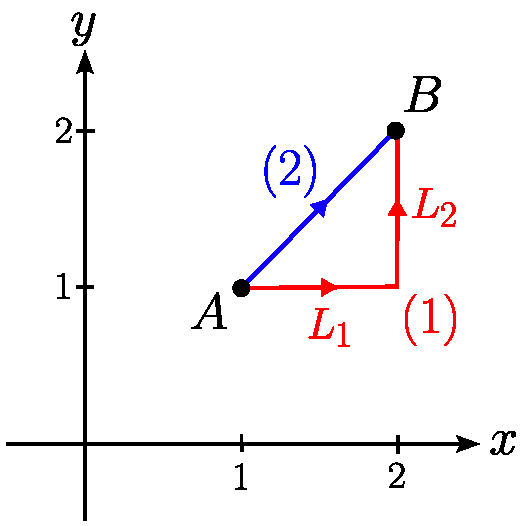
\includegraphics[scale = 0.55]{Figuras/Ej-Integral-Linea.pdf}
        \caption{Curva de integración.}
        \label{fig:Ej_Int_Linea}
    \end{figure}

    \textbf{Solución:} La trayectoria (1) se divide en dos partes. A lo largo del segmento horizontal $L_1$, no hay cambios en $y$ ni en $z$, entonces $dy = dz = 0$ y $d\Vec{x} = dx \hat{x}$. Además, a lo largo del segmento, $1 \leq x \leq 2$ e $y = 1$.

    Así,
    $$\int_{L_1} \Vec{F} \cdot d \Vec{x} = \int_1^2 ((1)^2 \hat{x} + 2x(1+1) \hat{y}) \cdot (dx \hat{x}) = \int_1^2 dx = 1.$$

    En el segmento vertical $L_2$, no hay cambios en $x$ ni en $z$, entonces $dx = dz = 0$ y $d\Vec{x} = dy \hat{y}$. Además, a lo largo de este segmento, $x = 2$ y $1 \leq y \leq 2$.

    Así,
    $$\int_{L_2} \Vec{F} \cdot d \Vec{x} = \int_1^2 (y^2 \hat{x} + 2(2)(y+1) \hat{y}) \cdot (dy \hat{y}) = \int_1^24(y+1) dy = 10.$$

    Por lo tanto, la integral de línea en torno a la trayectoria (1) es
    $$\int_A^B \Vec{F} \cdot d\Vec{x} = \int_{L_1} \Vec{F} \cdot d \Vec{x} + \int_{L_2} \Vec{F} \cdot d \Vec{x} = 11.$$

    Por otro lado, para la trayectoria (2), no hay cambios en $z$, así que $dz = 0$. Pero, $y = x$ y, en consecuencia,
    $$dx = dy \Rightarrow d\Vec{x} = dx \hat{x} + dy \hat{y} = dx \hat{x} + dx \hat{y} = (\hat{x} + \hat{y} ) dx.$$

    Hemos elegido la variable $x$ para integrar, lo cual es arbitrario (se llega al mismo resultado eligiendo $y$). Entonces,
    $$\int_A^B \Vec{F} \cdot d\Vec{x} = \int_1^2 (x^2 \hat{x} + 2x(x+1) \hat{y}) \cdot (\hat{x} + \hat{y} ) dx = \int_1^2 3x^2 + 2x \,dx = 10.$$
\end{ejemplo}

\textbf{Observaciones:}

\begin{enumerate}
    \item Las curvas del ejemplo estaban constituidas de segmentos y el campo vectorial estaba escrito en coordenadas $(x,y,z)$, lo cual facilitó el cálculo usando coordenadas cartesianas. Sin embargo, si se hubiese integrado, por ejemplo, sobre un arco de circunferencia, las coordenadas cartesianas dejan de ser útiles. Entonces, dependiendo de la curva y la forma del campo vectorial, se elige el sistema de coordenadas apropiado para atacar la integral.

    \item En general, las integrales de línea dependen de la trayectoria que unen los puntos.
\end{enumerate}


Un tipo de campo vectorial muy importante al momento de calcular integrales de línea son los campo \textbf{conservativos}. 

Un campo vectorial $\vec{F}$ se dice \textbf{conservativo} si existe un campo escalar $\phi$ tal que
\begin{equation*}
\vec{F} = \vec{\nabla} \phi.
\end{equation*}

De aquí se deriva el \textbf{teorema fundamental para gradientes}, el cual expresa que
\begin{shaded}
   \begin{equation*}
\int_A^B \vec{F} \cdot d\vec{r} = \int_A^B \Vec{\nabla} \phi \cdot d\Vec{x} = \phi(B) - \phi(A),
\end{equation*} 
\end{shaded}

para cualquier curva que una $A$ y $B$.

Si $\Vec{F}$ es un campo conservativo, se verifica:
\begin{enumerate}
\item $\int \vec{F} \cdot d\vec{r}$ es independiente de la trayectoria tomada.

\item $\oint\vec{F} \cdot d\vec{r} = 0$ para toda trayectoria cerrada.

\item $\vec{\nabla} \times \vec{F} = \vec{0}$, es decir, un campo conservativo es irrotacional.
\end{enumerate}

\subsection{Integrales de superficie}

Las integrales de superficie pueden tener las siguientes formas>
\begin{equation*}
\iint_S \phi d\vec{S}, \quad \iint_S \vec{F} \cdot d\vec{S}, \quad \iint_S \vec{F} \times d\vec{S},
\end{equation*}

donde $\phi$ es un campo escalar, $\vec{F}$ un campo vectorial y $d\vec{S}$ un vector de superficie infinitesimal de la superficie $S$ la cual puede ser abierta o cerrada. De nuevo, para superficies cerradas se usa el símbolo $\oiint$.

El elemento $d\vec{S}$ se define perpendicular a la superficie y a veces se escribe como $d\vec{S} = \hat{n} dS$, donde $\hat{n}$ es un vector unitario perpendicular a la superficie en la posición del elemento y $dS$ es la magnitud (escalar) de $d\vec{S}$. Si la superficie encierra un volumen, $\hat{n}$ apunta fuera del volumen (a menos que se indique lo contrario), ver figura \ref{fig:Superficies}-(a).

Para el caso de una superficie $S$ que no está en un volumen cerrado, diremos que la orientación de la curva cerrada $C$, trazada sobre el contorno de $S$, es compatible con la orientación de $S$ si la orientación de $C$ y $S$ cumplen con la regla de la mano derecha, ver figura \ref{fig:Superficies}-(b).

\begin{figure}[H]
    \centering
    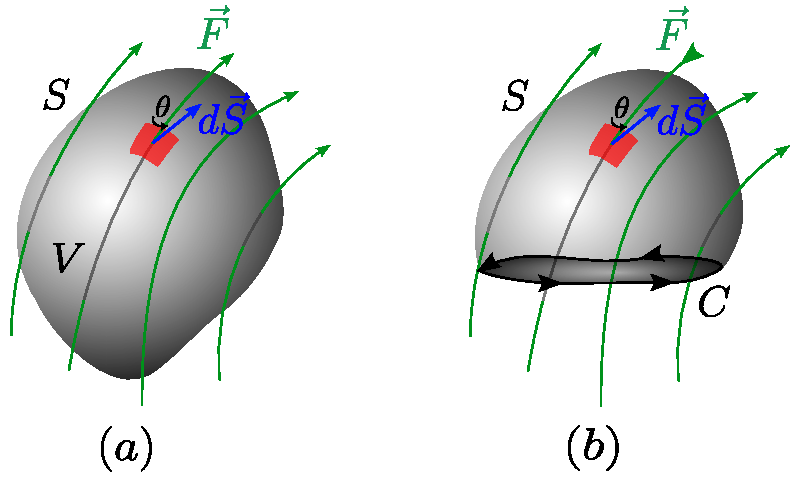
\includegraphics[scale = 0.8]{Figuras/ElementoSuperficie.pdf}
    \caption{En $(a)$ una superficie cerrada y en $(b)$ una superficie abierta. En cada caso se muestra un vector normal a la superficie $d\Vec{S}$, el cual forma un ánuglo $\theta$ con el campo vectorial $\Vec{F}$.}
    \label{fig:Superficies}
\end{figure}


Las integrales de superficie más comunes son las de tipo 
\begin{equation*}
\Phi_F = \iint_S \vec{F} \cdot d\vec{S},
\end{equation*}

llamadas integrales de \textbf{flujo}.

\begin{ejemplo}
    Calcule la integral de superficie de 
    $$\Vec{F}(x,y,z) = 2xz \hat{x} + (x+2) \hat{y} + y(z^2-3) \hat{z}$$

    sobre las cinco caras (no incluyendo la basal) de la caja cúbica en la figura \ref{fig:Ej_Int_Superficie}.

    \begin{figure}[H]
        \centering
        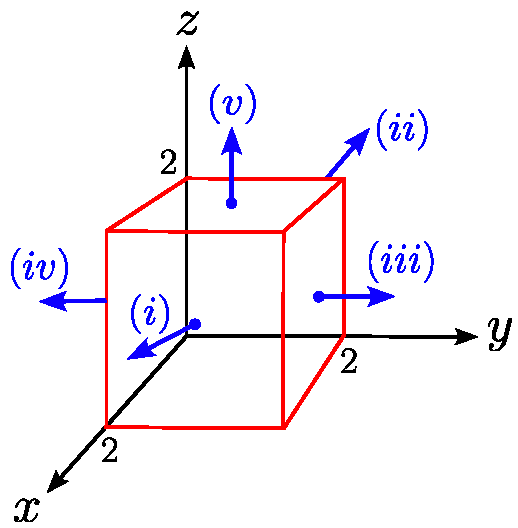
\includegraphics[scale = 0.7]{Figuras/Ej-Integral-Superficie.pdf}
        \caption{Superficie de integración.}
        \label{fig:Ej_Int_Superficie}
    \end{figure}

    \textbf{Solución:}  Tomando las caras una a la vez.

    \begin{itemize}
        \item[(i)] Para la cara $x = 2$, $d\Vec{S} = dydz \hat{x}$ con $0 \leq y \leq 2$ y $0 \leq z \leq 2$. Entonces,
        \begin{align*}
             \iint \Vec{F} \cdot d\Vec{S} &= \int_0^2 \int_0^2 (4z \hat{x} + (2+2) \hat{y} + y(z^2-3) \hat{z}) \cdot (dydz \hat{x})  \\
             &= \int_0^2 \left( \int_0^2 4z dy\right) dz\\
             &= 4 \int_0^2 z \left( \int_0^2 dy \right) dz \\
             &= 4 \int_0^2 2z \,dz \\
             &= 16.
        \end{align*}

        \item[(ii)] Para la cara $x = 0$, $d\Vec{S} = -dydz \hat{x}$ con $0 \leq y \leq 2$ y $0 \leq z \leq 2$. Entonces,
        \begin{align*}
             \iint \Vec{F} \cdot d\Vec{S} &= \int_0^2 \int_0^2 (0\hat{x} + (0+2) \hat{y} + y(z^2-3) \hat{z}) \cdot (-dydz \hat{x})  \\
             &= \int_0^2 \left( \int_0^2 0 \, dy\right) dz\\
             &= 0.
        \end{align*}

        \item[(iii)] Para la cara $y = 2$, $d\Vec{S} = dxdz \hat{y}$ con $0 \leq x \leq 2$ y $0 \leq z \leq 2$. Entonces,
        \begin{align*}
             \iint \Vec{F} \cdot d\Vec{S} &= \int_0^2 \int_0^2 (2xz \hat{x} + (x+2) \hat{y} + 2(z^2-3) \hat{z}) \cdot (dxdz \hat{y})  \\
             &= \int_0^2 \left( \int_0^2 x+2 \,dx\right) dz\\
             &=  \int_0^2   6 \, dz \\
             &= 12.
        \end{align*}

        \item[(iv)] Para la cara $y = 0$, $d\Vec{S} = -dxdz \hat{y}$ con $0 \leq x \leq 2$ y $0 \leq z \leq 2$. Entonces,
        \begin{align*}
             \iint \Vec{F} \cdot d\Vec{S} &= \int_0^2 \int_0^2 (2xz \hat{x} + (x+2) \hat{y} + 0 \hat{z}) \cdot (-dxdz \hat{y})  \\
             &=- \int_0^2 \left( \int_0^2 x+2 \, dx\right) dz\\
             &=  - 12.
        \end{align*}

        \item[(v)] Para la cara $z = 2$, $d\Vec{S} = dxdy \hat{z}$ con $0 \leq x \leq 2$ y $0 \leq y \leq 2$. Entonces,
        \begin{align*}
             \iint \Vec{F} \cdot d\Vec{S} &= \int_0^2 \int_0^2 (4x \hat{x} + (x+2) \hat{y} + y((2)^2-3) \hat{z}) \cdot (dxdy \hat{z})  \\
             &= \int_0^2 \left( \int_0^2 y\, dx\right) dy\\
             &= \int_0^2 2y\,dy \\
             &= 4.
        \end{align*}
    \end{itemize}

    Por lo tanto, el flujo total es
    $$\iint_S \Vec{F} \cdot d\Vec{S} = 16 + 0 + 12 - 12 + 4 = 20.$$
\end{ejemplo}

\textbf{Observación:} Al igual que para las integrales de líneas, la forma del campo vectorial y de la superficie permitió que la integral sea sencillamente calculada en coordenadas cartesianas, pero si nos enfrentamos a, por ejemplo, un cilindro, es conveniente utilizar otras coordenadas.

\subsection{Integral de volumen}

Una integral de volumen es una expresión de la forma
$$\iiint_V f(x,y,z) \,dV,$$

donde $f(x,y,z)$ es un campo escalar y $dV$ un elemento infinitesimal de volumen. En coordenadas cartesianas,
$$dV = dx dy dz.$$

Ocasionalmente nos encontraremos con integrales de volumen de campos vectoriales:
\begin{align*}
  \iiint_V \vec{F} dV &= \iiint_V (F_x \hat{x} + F_y \hat{y} + F_z \hat{z}) \,dV\\
  &=\hat{x} \iiint_V F_x dV +  \hat{y} \iiint_V F_y dV  + \hat{z} \iiint_V F_z dV, 
\end{align*}

porque los vectores unitarios ($\hat{x}$, $\hat{y}$ y $\hat{z}$) son constantes, salen de la integral.

\begin{ejemplo}
    Calcule la integral de volumen del campo escalar $f(x,y,z) = x^2$ sobre el tetraedro con vértices $(0,0,0)$, $(1,0,0)$, $(0,1,0)$ y $(0,0,1)$.

    \textbf{Solución:} La gráfica del tetraedro en conjunto con su proyección en el plano $xy$ se ilustra en la figura \ref{fig:Ej-Int_Volumen}.

    \begin{figure}[H]
        \centering
        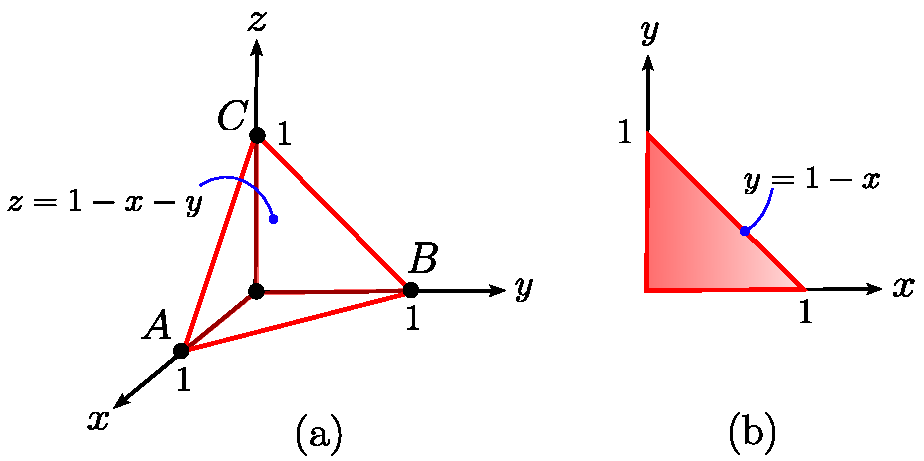
\includegraphics[scale = 0.7]{Figuras/Ej-Integral-Volumen.pdf}
        \caption{En (a) el tetraedro y en (b) la proyección (sombra) del tetraedro en el plano $xy$.}
        \label{fig:Ej-Int_Volumen}
    \end{figure}

    Determinemos la ecuación del plano que pasa por $A = (1,0,0)$, $B = (0,1,0)$ y $C = (0,0,1)$. Sean los vectores
    \begin{align*}
        \overrightarrow{CA} &= (1,0,0) - (0,0,1) = (1,0,-1), \\
        \overrightarrow{CB} &= (0,1,0) - (0,0,1) = (0,1,-1).
    \end{align*}

    Un vector normal al plano es
    $$\Vec{n} = \overrightarrow{CA} \times  \overrightarrow{CB} = (1,1,1).$$

    Entonces, la ecuación del plano está dada por
    $$\Vec{n} \cdot ( (x,y,z) - (1,0,0)) = 0 \Rightarrow x + y + z = 1.$$
    
    Para calcular este tipo de integrales debemos primero elegir un orden de integración, en nuestro caso será integrar en la variable $z$, luego en la variable $y$ y por último en la variable $x$, esto es, el orden $dzdydx$. Segundo, hay que establecer los límites de integración. Para $z$ imaginemos que tenemos un paralelepípedo de base $dydx$ (las variables que se integrarán después) y altura variable $z$, ver figura \ref{fig:Ej-Int_Volumen-2}-(a). Es claro que independiente donde se sitúe el paralelepípedo dentro del tetraedro, la variable $z$ se encuentra acotada inferiormente por el plano $z = 0$ y superiormente por el plano $z = 1 - x -y$, es decir,
    $$0 \leq z \leq 1-x-y.$$

    Ahora, para $y$, veamos la proyección del tetraedro en el plano $xy$, ver figura \ref{fig:Ej-Int_Volumen-2}-(b). Imaginemos que tenemos un rectángulo de base $dx$ (la variable que se integrará después) y altura variable $y$. Es claro que independiente donde se sitúe el rectángulo, la variable $y$ se encuentra acotada inferiormente por la recta $y = 0$ y superiormente por $y = 1 - x$, es decir,
    $$0 \leq y \leq 1-x.$$

    Finalmente, $x$ se desplaza entre $0$ y $1$, 
    $$0 \leq x \leq 1.$$

     \begin{figure}[H]
        \centering
        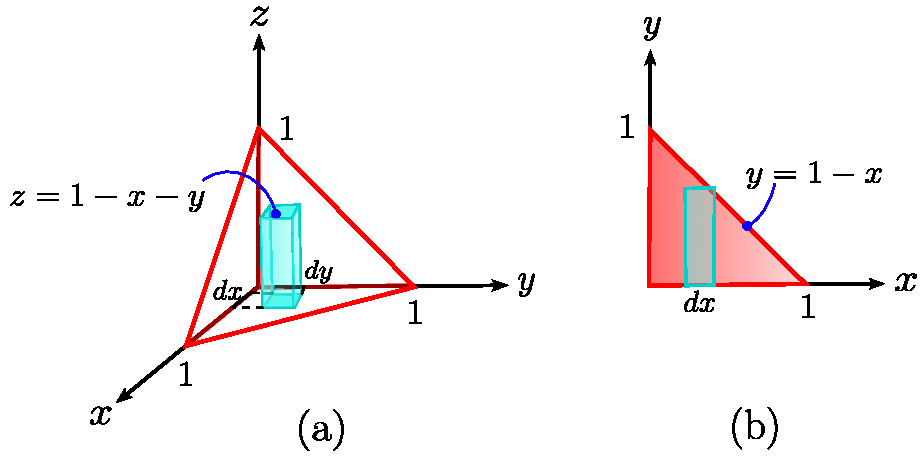
\includegraphics[scale = 0.7]{Figuras/Ej-Integral-Volumen-2.pdf}
        \caption{En (a) el tetraedro y en (b) la proyección  del tetraedro en el plano $xy$ en conjunto con el paralelepípedo y el rectángulo para ayudar a ver los límites de integración.}
        \label{fig:Ej-Int_Volumen-2}
    \end{figure}

    Por lo tanto,
    \begin{align*}
        \iiint_V x^2 \,dV &= \int_0^1 \left(\int_0^{1-x} \left(\int_0^{1-x-y} x^2 \,dz \right) dy \right) dx \\
        &= \int_0^1 \left(\int_0^{1-x} \left.  x^2 z \right|_{z=0}^{z = 1-x-y} dy \right) dx \\
        &= \int_0^1 \left(\int_0^{1-x} x^2(1-x-y) dy \right) dx \\
        &= \int_0^1 x^2 \left[ (1-x)y - \frac{y^2}{2} \right]_{y = 0}^{y = 1-x} dx  \\
        &= \int_0^1 x^2  (1-x)^2- x^2 \frac{(1-x)^2}{2}  \,dx \\
        &= \frac{1}{2} \int_0^1 x^2(1-x)^2 \,dx \\
        &= \frac{1}{60}.
    \end{align*}

    Queda como ejercicio para el lector verificar que para los órdenes de integración:
    \begin{enumerate}
        \item $dxdydz$:
        $$V: \left\{ \begin{array}{ccccl}
             0 & \leq & x & \leq & 1-z-y  \\
             0 & \leq & y & \leq & 1-z \\
             0 & \leq & z & \leq & 1
        \end{array} \right. .$$

        \item $dydzdx$:
        $$V: \left\{ \begin{array}{ccccl}
             0 & \leq & y & \leq & 1-z-x  \\
             0 & \leq & z & \leq & 1-x \\
             0 & \leq & x & \leq &1
        \end{array} \right. .$$
    \end{enumerate}

    se obtiene el mismo valor.
\end{ejemplo}

\subsection{Teoremas integrales}

\begin{teorema}[de Gauss] \label{Gauss}
    Sea $V$ una región limitada por una superficie $S$ suave y cerrada, tal que se le pueda atribuir una orientación en cada punto. Si $\vec{F}$ es un campo vectorial de clase $C^1$ sobre un abierto que contiene a $V$ y $\hat{n}$ la orientación dada por la normal exterior a $S$. Entonces,
    \begin{equation*}
    \boxed{\iint_S \vec{F} \cdot \hat{n}dS = \iiint_V \vec{\nabla} \cdot \vec{F} dV} 
    \end{equation*}
\end{teorema}

\begin{teorema}[de Stokes] \label{Stokes}
    Sea $S$ una superficie suave orientada con un vector unitario $\hat{n}$ y supongamos que $S$ tiene un borde $C$, que es una curva cerrada, lisa a trozos (seccionalmente suave), cuya orientación es compatible con la de $S$.

    Si $\vec{F}$ es un campo vectorial de clase $C^1$ en un abierto que contiene a $S$ y su frontera $C$, se verifica:
    \begin{equation*}
    \boxed{\int_C \vec{F} \cdot d\vec{r} = \iint_S (\vec{\nabla} \times \vec{F}) \cdot \hat{n}dS}
    \end{equation*}
\end{teorema}

\section{Coordenadas curvilíneas}

Las \textbf{coordenadas curvilíneas} son sistemas de coordenadas en el espacio Euclidiano donde las líneas coordenadas pueden ser curvas. Estas coordenadas pueden ser obtenidas a partir del sistema de coordenadas cartesiano mediante una transformación que es \underline{invertible} en cada punto. Esto significa que podemos convertir un punto dado en coordenadas cartesianas a un sistema curvilíneo y viceversa.

\subsection{Coordenadas esféricas}

Un punto $P$ en el espacio tridimensional euclídeo, en coordenadas esféricas, se especifica mediante tres coordenadas: $(r, \theta, \varphi)$, donde $r$ es la distancia desde el origen al punto $P$, $\theta$ es el ángulo que se forma entre el semieje $z$ positivo y el vector, y $\varphi$ es el ángulo que se forma entre el semieje $x$ positivo y la proyección del vector en el plano $xy$, ver figura \ref{fig:Coordenadas-Esfericas}.

\begin{figure}[H]
    \centering
    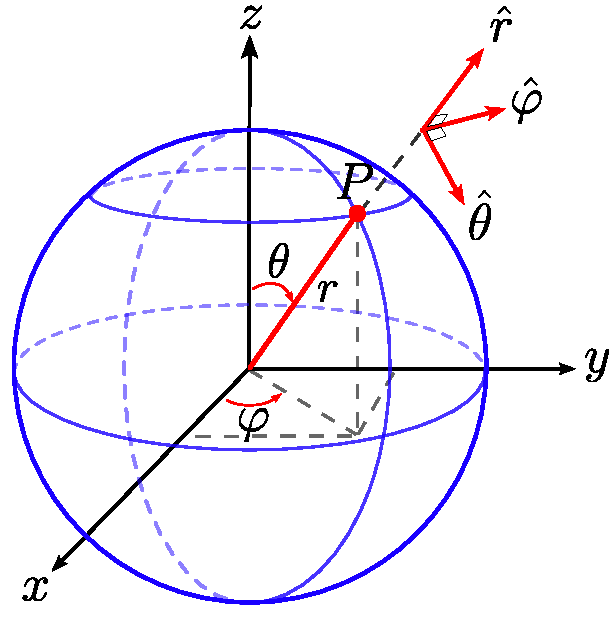
\includegraphics[scale = 0.65]{Figuras/Coordenadas-Esfericas.pdf}
    \caption{Coordenadas esféricas $(r,\theta,\varphi)$ en conjunto con sus vectores unitarios.}
    \label{fig:Coordenadas-Esfericas}
\end{figure}

Si se restringen las coordenadas $r$, $\theta$ y $\varphi$ a
\begin{equation}
r \geq 0, \quad 0 \leq \theta \leq \pi, \quad 0 \leq \varphi < 2\pi,
\end{equation}
se puede obtener todo punto $P \in \mathbb{R}^3$. Gracias a las restricciones, se tiene la siguiente conversión de coordenadas esféricas a cartesianas:
\begin{align}
    x &= r \sin \theta \cos \varphi,\\
    y &= r \sin \theta \sin \varphi ,\\
    z &= r \cos \theta,
\end{align}
y de cartesianas a esféricas\footnote{Recuerde que el recorrido de la función $\arccos(x)$ es $[-\pi/2, \pi/2]$ y de la función $\arctan(x)$ es $]-\pi/2, \pi/2[$, entonces dependiendo dónde se ubique $(x,y,z)$ se tendrá que sumar un múltiplo de $\pi$.}: 
\begin{align}
    r &= \sqrt{x^2+y^2+z^2}, \\
    \theta &= \arccos \left(\frac{z}{r} \right) = \arccos \left( \frac{z}{\sqrt{x^2+y^2+z^2}} \right), \\
    \varphi &= \arctan \left( \frac{y}{x} \right).
\end{align}

La base ortonormal en el sistema de coordenadas esféricas la forman los vectores $\hat{r}, \hat{\theta}$ y $\hat{\varphi}$, ver figura \ref{fig:Coordenadas-Esfericas}, los cuales apuntan en el sentido de crecimiento de las correspondientes coordenadas y verifican
\begin{equation}
\hat{\theta} \times \hat{\varphi} = \hat{r}.
\end{equation}

Al igual que toda base, todo vector $\Vec{A}$ puede ser expresado en términos de ellos, en la forma usual:
\begin{equation}
\Vec{A} = A_r \hat{r} + A_{\theta} \hat{\theta} + A_{\varphi} \hat{\varphi}.
\end{equation}
A partir de la transformación de coordenadas, el vector posición toma la forma
\begin{equation}
\Vec{x} = x \,\hat{x} + y \,\hat{y} + z \,\hat{z} = r \sin \theta \cos \varphi \,\hat{x} + r \sin \theta \sin \varphi \,\hat{y} + r \cos\theta \,\hat{z}.
\end{equation}

Así, los vectores unitarios pueden ser expresados en la base cartesiana $\{\hat{x}, \hat{y}, \hat{z}\}$, como sigue:
\begin{align}
    \hat{r} &= \frac{1}{\norm{\frac{\partial \Vec{x}}{\partial r}}}\frac{\partial \Vec{x}}{\partial r} = \sin \theta \cos \varphi \,\hat{x} + \sin \theta \sin \varphi \,\hat{y} + \cos \theta \,\hat{z}, \label{rxyz} \\
    \hat{\theta} &= \frac{1}{\norm{\frac{\partial \Vec{x}}{\partial \theta}}}\frac{\partial \Vec{x}}{\partial \theta} = \cos \theta \cos \varphi \,\hat{x} + \cos \theta \sin \varphi \,\hat{y} - \sin \theta   \,\hat{z},  \\
    \hat{\varphi} &= \frac{1}{\norm{\frac{\partial \Vec{x}}{\partial \varphi}}}\frac{\partial \Vec{x}}{\partial \varphi} = - \sin \varphi \,\hat{x} + \cos \varphi \,\hat{y} . \label{varphixyz}
\end{align}

\textbf{Nota:} Dado que la derivada parcial con respecto a una coordenada considera el resto como constantes, el vector unitario es tangente a la curva que se genera manteniendo dichas coordenadas constantes. Por ejemplo, $\hat{r}$ es tangente a la curva que se genera al considerar $\theta$ y $\varphi$ constantes, esto es, un rayo que parte del origen.

Observe que los vectores unitarios $\hat{r}, \hat{\theta}$ y $\hat{\varphi}$ \textit{no son constantes}, a diferencia de los vectores unitarios cartesianos, de hecho $\hat{r} = \hat{r}(\theta,\varphi)$, $\hat{\theta} = \hat{\theta}(\theta,\varphi)$ y $\hat{\varphi} = \hat{\varphi}(\theta,\varphi)$. Por lo tanto, al momento de derivar o integrar hay que tener cuidado.

Por lo anterior, el vector posición de un punto $P$ con coordenadas $(r, \theta, \varphi)$ es dado por
\begin{equation}
\vec{x} = r \hat{r}
\end{equation}
La relación inversa a \eqref{rxyz}--\eqref{varphixyz}, es decir, la expresión de los vectores unitarios cartesianos en términos de los vectores unitarios esféricos, es dada por
\begin{align}
    \hat{x} &= \sin \theta \cos \varphi \,\hat{r} + \cos \theta \cos \varphi \,\hat{\theta} - \sin \varphi \,\hat{\varphi},\\
    \hat{y} &= \sin \theta \sin\varphi \,\hat{r} + \cos \theta \sin \varphi \,\hat{\theta} + \cos \varphi \,\hat{\varphi}, \\
    \hat{z} &= \cos \theta \,\hat{r} - \sin \theta \,\hat{\theta}.
\end{align}

Consideremos un punto $(r,\theta, \varphi)$ en el espacio, nos desplazamos infinitesimalmente en las direcciones $\hat{r}$, $\hat{\theta}$ y $\hat{\varphi}$ al punto $(r + dr, \theta + d\theta, \varphi + d\varphi)$. El desplazamiento infinitesimal general está dado por
\begin{shaded}
    $$d\Vec{x} = dr \, \hat{r} + r \,d\theta \,\hat{\theta} + r \sin \theta \,d\varphi \,\hat{\varphi}.$$
\end{shaded}

\begin{figure}[H]
    \centering
    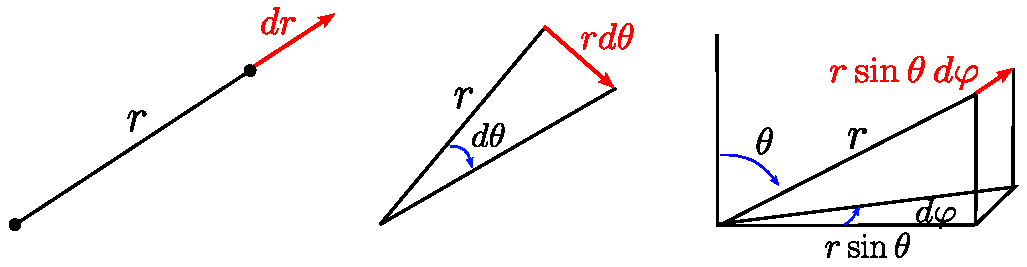
\includegraphics[scale = 0.7]{Figuras/Elemento-Esferica.pdf}
    \caption{}
    \label{fig:Elemento-Esferica}
\end{figure}

El elemento infinitesimal de volumen, en coordenadas esféricas, es el producto de los tres desplazamientos infinitesimales:
\begin{shaded}
\begin{equation}
dV = r^2 \sin \theta \,dr\,d\theta\,d\varphi,
\end{equation}
\end{shaded}
lo cual corresponde al volumen del paralelepípedo formado por los vectores: $dr \,\hat{r}$, $r \,d\theta \, \hat{\theta}$ y $r \sin \theta \,d\varphi \, \hat{\varphi}$.

No existe una expresión general para los elementos de superficie $d\Vec{S}$, ya que estos dependen de la orientación de la superficie. Para obtenerlos uno tiene que analizar la geometría para cada caso. En la figura \ref{fig:Vol-Esfericas}, se encuentran representados los diferentes elementos infinitesimales que se pueden obtener. Para el caso de los elementos infinitesimales  de superficie, se tienen tres casos:
\begin{shaded}
  \begin{equation*}
d\vec{S}_r = r^2 \sin \theta\, d\theta\, d\varphi \,\hat{r} ,\quad d\vec{S}_{\theta} = r \sin\theta \,dr \,d \varphi \,\hat{\theta}, \quad  d\vec{S}_{\varphi} = r \,dr\, d\theta \,\hat{\varphi}.
\end{equation*}  
\end{shaded}

\begin{ejemplo}
    El volumen de una esfera (maciza) de radio $R$ es 
    \begin{align*}
        V = \int dV &= \int_0^{2\pi} \left( \int_0^{\pi} \left( \int_0^R r^2 \sin \theta \,dr \right)d\theta \right) d\varphi \\
        &= \left( \int_0^{2\pi} d\varphi\right) \left(\int_0^{\pi} \sin \theta \,d\theta \right) \left(\int_0^R r^2 \,dr \right) \\
        &= (2\pi) (2) \left(\frac{R^3}{3} \right) = \frac{4}{3} \pi R^3.
    \end{align*}
\end{ejemplo}

\begin{figure}[H]
    \centering
    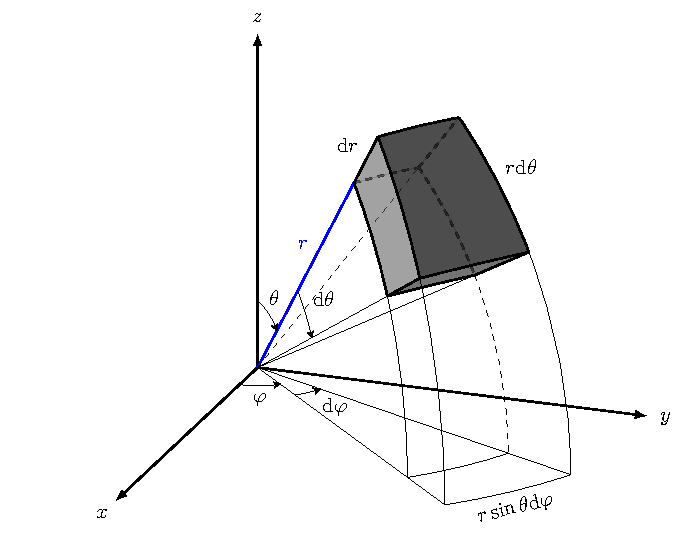
\includegraphics[scale = 1]{Figuras/volumen-esfericas.pdf}
    \caption{Elementos infinitesimales en coordenadas esféricas. Adaptado a partir de versión de A. Tsagkaropoulos, disponible en \href{https://tikz.net/spherical_volume/}{esta página}.}
    \label{fig:Vol-Esfericas}
\end{figure}

\subsection{Coordenadas cilíndricas}

Un punto $P$ en el espacio tridimensional euclídeo, en coordenadas cilíndricas, se especifica mediante tres coordenadas: $(\rho, \varphi, z)$, donde $\rho$ es la distancia a $P$ desde el eje $z$, $\varphi$ es el ángulo que se forma entre el semieje $x$ positivo y la proyección del vector en el plano $xy$, y $z$ es la misma coordenada que en cartesianas, ver figura \ref{fig:Coordenadas-Cilindricas}.

\begin{figure}[H]
    \centering
    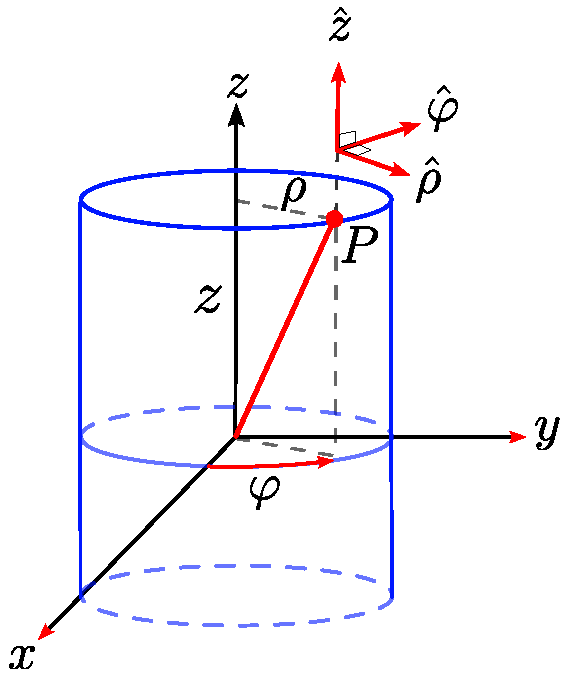
\includegraphics[scale = 0.7]{Figuras/Coordenadas-Cilindricas.pdf}
    \caption{Coordenadas cilíndricas $(\rho,\varphi, z)$ en conjunto con sus vectores unitarios.}
    \label{fig:Coordenadas-Cilindricas}
\end{figure}

Si se restringen las coordenadas $\rho$, $\varphi$ y $z$ a
\begin{equation}
\rho \geq 0, \quad 0 \leq \varphi < 2\pi, \quad -\infty < z < \infty,
\end{equation}
se puede obtener todo punto $P \in \mathbb{R}^3$. Gracias a las restricciones, se tiene la siguiente conversión de coordenadas cilíndricas a cartesianas:
\begin{align}
    x &= \rho \cos \varphi,\\
    y &= \rho \sin \varphi ,\\
    z &= z,
\end{align}
y de cartesianas a cilíndricas:
\begin{align}
    \rho &= \sqrt{x^2+y^2}, \\
    \varphi &= \arctan \left( \frac{y}{x} \right), \\
    z &= z .
\end{align}

La base ortonormal en el sistema de coordenadas cilíndricas la forman los vectores $\hat{\rho}, \hat{\varphi}$ y $\hat{z}$, ver figura \ref{fig:Coordenadas-Cilindricas}, que verifican:
\begin{equation}
\hat{\rho} \times \hat{\varphi} = \hat{z}.
\end{equation}


Un vector $\Vec{A}$ puede ser expresado en términos de ellos, en la forma usual:
\begin{equation}
\Vec{A} = A_{\rho} \hat{\rho}  + A_{\varphi} \hat{\varphi} + A_z \hat{z}.
\end{equation}

A partir de la transformación de coordenadas, el vector posición toma la forma
\begin{equation}
\Vec{x} = x \,\hat{x} + y \,\hat{y} + z \,\hat{z} = \rho \cos \varphi \,\hat{x} + \rho \sin \varphi \,\hat{y} + z \,\hat{z}.
\end{equation}

Así, los vectores unitarios pueden ser expresados en la base cartesiana $\{\hat{x}, \hat{y}, \hat{z}\}$, como sigue.
\begin{align}
    \hat{\rho} &= \frac{1}{\norm{\frac{\partial \Vec{x}}{\partial \rho}}}\frac{\partial \Vec{x}}{\partial \rho} = \cos \varphi \,\hat{x} + \sin \varphi \,\hat{y}, \\
    \hat{\varphi} &= \frac{1}{\norm{\frac{\partial \Vec{x}}{\partial \varphi}}}\frac{\partial \Vec{x}}{\partial \varphi} = - \sin \varphi \,\hat{x} + \cos \varphi \, \hat{y},  \\
    \hat{z} &= \frac{1}{\norm{\frac{\partial \Vec{x}}{\partial z}}}\frac{\partial \Vec{x}}{\partial z} = \hat{z} .
\end{align}

Por lo anterior, el vector posición de un punto $P$ con coordenadas $(\rho, \varphi,z)$ es 
\begin{equation}
\vec{x} = \rho \hat{\rho} + z \hat{z}.
\end{equation}

Se puede demostrar que los vectores unitarios cartesianos se pueden escribir como combinación lineal de los vectores unitarios cilíndricos, a saber:
\begin{align}
    \hat{x} &= \cos \varphi \,\hat{\rho} - \sin \varphi \, \hat{\varphi}, \\
    \hat{y} &= \sin\varphi \, \hat{\rho} + \cos \varphi \,\hat{\varphi}.
\end{align}

Consideremos un punto $(\rho, \varphi, z)$ en el espacio, nos desplazamos infinitesimalmente en las direcciones $\hat{\rho}$, $\hat{\varphi}$ y $\hat{z}$ al punto $(\rho + d\rho, \varphi + d\varphi, z + dz)$. A partir de la figura \ref{fig:Elemento-Cilindrica}, se tiene que los elementos infinitesimales de longitud en las direcciones $\hat{\rho}$, $\hat{\varphi}$ y $\hat{z}$, están dados, respectivamente, por
\begin{equation}
dx_{\rho} = d\rho, \quad dx_{\varphi} = \rho \,d\varphi, \quad dx_z = dz.
\end{equation}

Por lo tanto, el desplazamiento infinitesimal general está dado por
\begin{shaded}
\begin{equation}
d\Vec{x} = d\rho \, \hat{\rho} + \rho \,d\varphi \,\hat{\varphi} + dz \,\hat{z}.
\end{equation}
\end{shaded}

\begin{figure}[H]
    \centering
    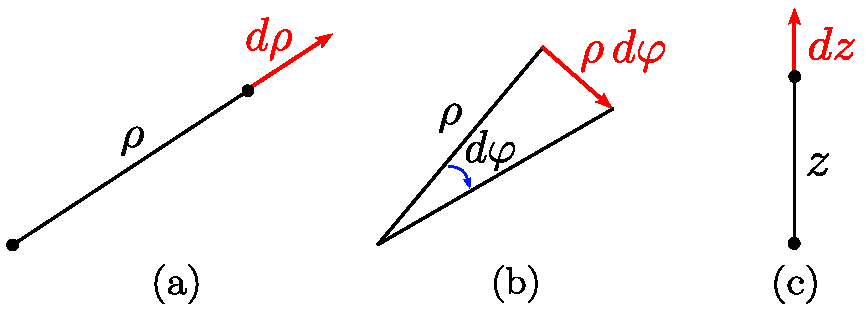
\includegraphics[scale = 0.7]{Figuras/Elemento-Cilindrica.pdf}
    \caption{}
    \label{fig:Elemento-Cilindrica}
\end{figure}

El elemento infinitesimal de volumen, en coordenadas cilíndricas, es el producto de los tres desplazamientos infinitesimales:
\begin{shaded}
\begin{equation}
dV = \rho \,d\rho\,d\varphi\,dz,
\end{equation}
\end{shaded}
lo cual corresponde al volumen del paralelepípedo formado por los vectores: $d\rho \hat{\rho}$, $\rho \,d\varphi \, \hat{\varphi}$ y $dz \, \hat{z}$.

 En la figura \ref{fig:Vol-Cilindricas}, se encuentran representados los diferentes elementos infinitesimales que se pueden obtener. Para el caso de los elementos infinitesimales  de superficie, se tienen tres casos:
\begin{shaded}
\begin{equation}
d\vec{S}_{\rho} = \rho \,d\varphi \,dz \,\hat{\rho},\quad d\vec{S}_{z} = \rho \,d\varphi\, d\rho \,\hat{z},\quad d\vec{S}_{\varphi} = d\rho\, dz \,\hat{\varphi}.
\end{equation}  
\end{shaded}

\begin{figure}[H]
    \centering
    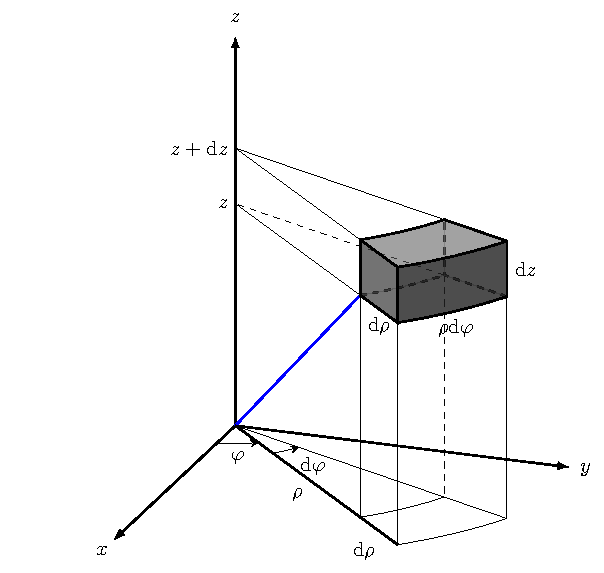
\includegraphics[scale = 1]{Figuras/volumen-cilindricas.pdf}
    \caption{Elementos infinitesimales en coordenadas cilíndricas. Adaptado a partir de versión de A. Tsagkaropoulos, disponible en \href{https://tikz.net/cylindrical_volume/}{esta página}.}
    \label{fig:Vol-Cilindricas}
\end{figure}

\section{Operadores en coordenadas curvilíneas}

En la sección \ref{Operadores} definimos los operadores vectoriales en coordenadas cartesianas. Ahora veremos la forma que tienen en coordenadas esféricas y cilíndricas.

Sea el campo escalar diferenciable $f$ y el campo vectorial diferenciable $\vec{F}$ de componentes $F_{\rho}, F_{\varphi}, F_z$ en coordenadas cilíndricas y de componentes $F_r, F_{\theta}, F_{\varphi}$  en coordenadas esféricas.

\begin{itemize}
\item[i)] El \textbf{gradiente} en coordenadas cilíndricas es
\begin{shaded}
\begin{equation}
\vec{\nabla} f(\rho, \varphi,z) = \frac{\partial f}{\partial \rho} (\rho, \varphi, z) \hat{\rho} + \frac{1}{\rho}  \frac{\partial f}{\partial \varphi} (\rho, \varphi, z) \hat{\varphi} + \frac{\partial f}{\partial z} (\rho, \varphi, z) \hat{z},
\end{equation}
\end{shaded}
y en coordenadas esféricas
\begin{shaded}
\begin{equation}
\vec{\nabla} f(r, \theta,\varphi) = \frac{\partial f}{\partial r} (r, \theta, \varphi) \hat{r} + \frac{1}{r} \frac{\partial f}{\partial \theta}(r, \theta, \varphi) \hat{\theta} + \frac{1}{r\sin\theta}\frac{\partial f}{\partial \varphi}(r, \theta, \varphi) \hat{\varphi}.
\end{equation}
\end{shaded}

\item[ii)] La \textbf{divergencia} en coordenadas cilíndricas es
\begin{shaded}
\begin{equation}
\vec{\nabla} \cdot \vec{F}(\rho, \varphi,z) = \frac{1}{\rho} \frac{\partial(\rho F_{\rho})}{\partial \rho} + \frac{1}{\rho} \frac{\partial F{\varphi}}{\partial\varphi} + \frac{\partial F_z}{\partial z},
\end{equation}
\end{shaded}
y en coordenadas esféricas
\begin{shaded}
\begin{equation}
\vec{\nabla} \cdot \vec{F}(r,\theta, \varphi) = \frac{1}{r^2} \frac{\partial (r^2 F_r)}{\partial r} + \frac{1}{r\sin\theta} \frac{\partial (\sin\theta F_{\theta})}{\partial \theta} + \frac{1}{r\sin\theta} \frac{\partial F_{\varphi}}{\partial \varphi}.
\end{equation}
\end{shaded}

\item[iii)] El \textbf{rotacional} en coordenadas cilíndricas es
\begin{shaded}
\begin{equation}
\vec{\nabla} \times \vec{F} = \left( \frac{1}{\rho} \frac{\partial F_z}{\partial \varphi} - \frac{\partial F_{\varphi}}{\partial z}\right) \hat{\rho} + \left( \frac{\partial F_{\rho}}{\partial z} - \frac{\partial F_z}{\partial \rho}\right) \hat{\varphi} + \frac{1}{\rho} \left[ \frac{\partial (\rho F_{\varphi})}{\partial \rho} - \frac{\partial F_{\rho}}{\partial \varphi} \right] \hat{z},
\end{equation}
\end{shaded}
y en coordenadas esféricas
\begin{shaded}
\begin{equation}
\vec{\nabla} \times \vec{F} = \frac{1}{r \sin \theta} \left[ \frac{\partial (\sin\theta F_{\varphi})}{\partial \theta} - \frac{\partial F_{\theta}}{\partial \varphi} \right]\hat{r} + \frac{1}{r} \left[ \frac{1}{\sin \theta} \frac{\partial F_r}{\partial \varphi} - \frac{\partial (r F_{\varphi})}{\partial r} \right] \hat{\theta} 
     + \frac{1}{r} \left[ \frac{\partial (rF_{\theta})}{\partial r} - \frac{\partial F_r}{\partial \theta} \right] \hat{\varphi}.
\end{equation}
\end{shaded}

\item[iv)] El \textbf{laplaciano} en coordenadas cilíndricas es
\begin{shaded}
\begin{equation}
\nabla^2 f(\rho, \varphi,z) = \frac{1}{\rho} \frac{\partial}{\partial \rho} \left(\rho \frac{\partial f}{\partial \rho} \right) + \frac{1}{\rho^2} \frac{\partial^2 f}{\partial \varphi^2}  + \frac{\partial^2 f}{\partial z^2},
\end{equation}
\end{shaded}
y en coordenadas esféricas
\begin{shaded}
\begin{equation}
\nabla^2 f(r,\theta,\varphi) = \frac{1}{r^2} \frac{\partial}{\partial r^2} \left( r^2 \frac{\partial f}{\partial r} \right) + \frac{1}{r^2 \sin\theta} \frac{\partial}{\partial \theta} \left( \sin \theta \frac{\partial f}{\partial \theta}\right) + \frac{1}{r^2 \sin^2\theta} \frac{\partial^2 f}{\partial \varphi^2}.
\end{equation}
\end{shaded}
\end{itemize}




